% Main-text body.  Five-page limit: the figure, five tables, six displayed
% equations, the abstract and nineteen headings cost ~2.2 pages, so the prose
% budget is ~1,850 words.  Detail lives in the appendix, which does not count.
% Check with:  ../.venv/Scripts/python.exe tools/prosecount.py
%             ../.venv/Scripts/python.exe tools/pagecheck.py

\maketitle

\begin{abstract}
A design campaign accepts every sample inside a tolerance band around a target, and we
study what limits that fraction under inference-time guidance. On QM9 3D coordinates we
train an E(3)-equivariant flow-matching model, compare it against a diffusion model,
and confirm guidance works, roughly doubling coverage while molecule stability falls
from $0.434$ to $0.246$. The property error splits into centring and spread: at a
median target centring is small relative to the band while spread is several band
widths, and one strength dial moves both. Batch-Dispersion Guidance measures the batch
spread of the guide's endpoint prediction, forms a scale-free error against a requested
setpoint, and servoes the guidance term's deviation gain by it while holding the
centring gain fixed, at no additional network evaluations. The setpoint moves achieved
spread monotonically on six of six property curves, from $0.67$ to $1.22$ times
unguided, including widening, which the strength dial does not reach. Coverage does not
improve over a tuned plug-in baseline: the coefficient is affine in the predicted
property, so the rule is the plug-in field reweighted.
Transferred unchanged to the probability simplex, every signature reproduces at a
smaller measured effect. The controller buys calibrated spread and chemical fidelity at
matched coverage.
\end{abstract}

\section{Introduction}

Continuous generative models learn a transport from a simple reference distribution to
a complex one. Diffusion reverses a stochastic corruption \citep{karras2022elucidating}
and flow matching regresses a vector field along a prescribed path
\citep{lipman2022flow}; stochastic interpolants contain both
\citep{albergo2025stochastic}, so one backbone serves either and the choice is
empirical. Can a frozen property predictor steer a pretrained generator?

A design campaign accepts any molecule inside a tolerance band. At a median target our
batches sit one or two band widths from the target while their spread is five to nine
band widths, so clustering limits coverage. Every guidance rule exposes one strength
dial moving centring and spread together \citep{ho2022classifier,zheng2023guided};
recent work makes that scale state dependent \citep{fbg2025feedback,cfgctrl2026} and
couples trajectories repulsively \citep{corso2024particle}, and none lets the user
request a spread in property units.

We ask one question on two state spaces: does making batch dispersion a requested
quantity raise band coverage? Modality 1 is QM9 3D coordinates and Modality 2 is DNA
enhancers on the probability simplex, and we expect a calibrated spread knob to raise
coverage and to transfer, since the controller reads a scalar variance carrying no
geometry.
\begin{itemize}[leftmargin=1.1em,itemsep=0pt,topsep=1pt,parsep=0pt]
  \item We compare flow matching and diffusion under one split, evaluator and budget.
  \item We demonstrate guidance against a matched unguided control and price it.
  \item We introduce BDG, servoing the deviation gain by the batch variance of the
    guide's own endpoint prediction at no extra network evaluations, and state the
    reduction bounding it.
  \item We transfer the controller to the simplex and test whether it generalizes.
\end{itemize}

\section{Related Work}

\textbf{Continuous models and guidance.} Flow matching \citep{lipman2022flow},
rectified flow \citep{liu2022flow} and EDM \citep{karras2022elucidating} are endpoints
of one construction \citep{albergo2025stochastic,ma2024sit}. Our five comparators are
DPS \citep{chung2023dps}, LGD-MC \citep{song2023lgd}, TMPD \citep{boys2024tmpd}, TFG
\citep{ye2024tfg} and D-Flow \citep{benhamu2024dflow}.

\textbf{Near our mechanism.} Prior work drives ensemble moments to a target
\citep{mgd2026moment}, tilts or aligns ensemble variance
\citep{vtd2026variance,ensemblevar2025}, couples trajectories
repulsively \citep{corso2024particle}, widens through negative guidance
\citep{ventura2026negative}, and reads the guidance scale as a control gain
\citep{cfgctrl2026,fbg2025feedback}. Over roughly eight queries we did not find a
weight set by the batch variance of a \emph{learned predictor's} endpoint prediction
against a \emph{two-sided user-chosen} setpoint.

\textbf{The two modalities.} EDM defines the stability conventions we adopt
\citep{hoogeboom2022equivariant}; see also
\citep{xu2022geodiff,irwin2024semlaflow,song2023equifm,bao2023eegsde}. On the simplex,
Dirichlet \citep{stark2024dirichlet}, Fisher \citep{davis2024fisher} and Gumbel-Softmax
\citep{tang2025gumbel} flow matching and MOG-DFM \citep{chen2025mogdfm} define the task
and score it by Fr\'echet biological distance at 500 base pairs.

\section{Methods}

\subsection{Modalities, Data, and Preprocessing}
\label{sec:data}

\textbf{Modality 1} is QM9, 133{,}885 molecules on $\mathbb{R}^{N\times3}$: at most 29
atoms, coordinates zero-centred, a hard one-hot over $\{$H,C,N,O,F$\}$, no feature
scaling. Splits are \texttt{train\_a} (51{,}527) for the generator and guide $f_A$,
\texttt{train\_b} (51{,}527) for the evaluator $f_B$, \texttt{val} (17{,}748) for
selection, \texttt{test} (13{,}083) held out, so scoring is independent of the guide.
Generation is unconditional, and the properties are dipole, polarizability and gap.

\textbf{Modality 2} is 6{,}126 \emph{Drosophila} Kenyon-cell enhancer regions on
$(\Delta^3)^L$, decoded by per-position $\arg\max$, a state space with no rotation
group and an exact property.

\subsection{Continuous Flow Matching Baseline}
\label{sec:fm}

With $t:0\to1$ from noise to data, the linear interpolant $x_t = t x_1 + (1-t) x_0$ has
constant conditional velocity $u_t=x_1-x_0$, and the source is projected onto the
zero-centre-of-mass subspace of dimension $3(N-1)$. The objective is a masked mean over
$t\sim\mathcal{U}(0,1)$, coordinates and types normalised separately, $\lambda=1$:
\begin{equation}
\mathcal{L}_{\mathrm{FM}}(\theta)=
\mathbb{E}_{t,x_0,x_1}\!\left[
\tfrac{1}{3\Sigma M}\big\|M\odot(v^{c}_\theta - u^{c})\big\|^2
+\lambda\tfrac{1}{K\Sigma M}\big\|M\odot(v^{f}_\theta - u^{f})\big\|^2
\right],
\label{eq:fmloss}
\end{equation}
with $M$ the atom mask and $K$ the type channels. The network is a dense
E($n$)-equivariant graph network, width 256, 8 layers, 3.75\,M parameters, Adam at
$2\times10^{-4}$, batch 256, EMA 0.9999, 1500 epochs (303k steps), selected on
validation atom stability. Sampling is explicit Euler, 100 steps.

\subsection{Diffusion Baseline}
\label{sec:diff}

The diffusion baseline shares everything with Section~\ref{sec:fm} but the corruption,
which makes Section~\ref{sec:fmvd} interpretable: a variance-preserving process with
$\beta(\tau)=\beta_{\min}+\tau(\beta_{\max}-\beta_{\min})$, $\beta_{\min}=0.1$,
$\beta_{\max}=20$:
\begin{equation}
x_\tau=\alpha(\tau)x_0+\sigma(\tau)\epsilon,
\quad
\log\alpha(\tau)=-\tfrac12\big(\beta_{\min}\tau+\tfrac12(\beta_{\max}-\beta_{\min})\tau^2\big),
\quad \alpha^2+\sigma^2=1 .
\label{eq:vp}
\end{equation}
The network predicts $\epsilon$. We integrate
$\mathrm{d}x/\mathrm{d}\tau=-\tfrac12\beta(\tau)(x+s_\theta)$ backwards,
$s_\theta=-\epsilon_\theta/\sigma$, on a decreasing 100-step grid, then jump to the
Tweedie mean: budget 101 against the flow model's 100.

\subsection{Guided Generation}
\label{sec:guidance}

Each guided step toward target $y$ forms the endpoint estimate $m_i$, which is
$x_t^{(i)}+(1-t)v_\theta(x_t^{(i)},t)$ for the flow model and the Tweedie mean for the
diffusion model, evaluates $F_i=f_A(m_i)$ and $g_i=\nabla_m f_A(m_i)$, and adds
\begin{equation}
G_i \;=\; \frac{\mathrm{num}_i}{s^2}\,J_i^{\!\top} g_i ,
\qquad
\mathrm{num}_i^{\mathrm{plug}} \;=\; y - F_i ,
\label{eq:plug}
\end{equation}
with $J_i^{\!\top}$ the vector-Jacobian product and $s$ the guide's target standard
deviation. The sampler scales this by $w(1-t)/t$ and applies a velocity-relative trust
region: removing it produces 222 non-finite samples against none clipped. Guidance runs
for $t\ge0.5$.

\subsection{Proposed Innovation: Batch-Dispersion Guidance}
\label{sec:bdg}

\textbf{Mechanism.} For a batch BDG forms the mean $\Fbar$, the unbiased variance $\Vb$
and the scale-free error $e=(\Vb-\tau^2)/\tau^2$ against a setpoint $\tau$, then
replaces the numerator of Equation~\eqref{eq:plug} by
\begin{equation}
\mathrm{num}_i \;=\; (y-F_i)\;-\;\eta\,e\,\big(F_i-\Fbar\big)
\;=\;\big(y-\Fbar\big)-\weff\big(F_i-\Fbar\big),
\qquad \weff=1+\eta e .
\label{eq:bdgnum}
\end{equation}
$\Vb>\tau^2$ contracts the batch and $\Vb<\tau^2$ expands it; both terms multiply the
same $g_i$, so BDG costs what plug-in costs. Algorithm~\ref{alg:bdg} is the whole step
and Figure~\ref{fig:mechanism} is it measured.

\textbf{The reduction.} Equation~\eqref{eq:bdgnum} is affine in $F_i$, so it factors
exactly,
\begin{equation}
(y-F_i)-\eta e\big(F_i-\Fbar\big)=\big(1+\eta e\big)\big(y_{\mathrm{eff}}-F_i\big),
\qquad
y_{\mathrm{eff}}=\frac{y+\eta e\,\Fbar}{1+\eta e},
\label{eq:reduction}
\end{equation}
verified to $3.0\times10^{-15}$ analytically and $6.5\times10^{-7}$ on the real field.
BDG is therefore the plug-in field at a rescaled weight aiming at a shifted target.

\textbf{Properties and controls.} Since $\Vb\ge0$, $\weff\ge1-\eta$ for any batch,
licensing two-sided operation and forcing $\eta>1$. A per-sample posterior variance
with $k=(1-t)^2/t$ fires its expansion branch unconditionally and must be clamped. The
equilibrium $V^{\star}=\tau^2(1-1/\eta)$ is an asymptote the 50-step window does not
reach, so we never describe $\tau$ as a value the sampler attains. Two settings are
\emph{gates}, not controls: $\eta=0$ and the one-sided variant must each reproduce the
plug-in field bit-identically. Three controls isolate the mechanism: a strength sweep
at fixed $(\eta,\tau)$, an open-loop replay of a recorded $e$ schedule on another seed,
and a matched signed-$w$ plug-in control, under a drop rule: if it reaches BDG's spread
at equal chemistry, the claim is withdrawn.

\subsection{Transfer to Modality 2}
\label{sec:transfer}

BDG's step is a per-sample scalar times the plug-in step, so it needs no inverse, which
matters where $\mathrm{diag}(p)-pp^\top$ is singular. What changes is the state space,
the generator and the property map, an analytic relaxation of GC content whose exact
count is the evaluator.

\subsection{Model Overview}
\label{sec:overview}

Figure~\ref{fig:overview} shows the whole study: the two base models, the guidance
signal, the component BDG changes, and what transfers to Modality 2.

\begin{figure}[!tb]
  \centering
  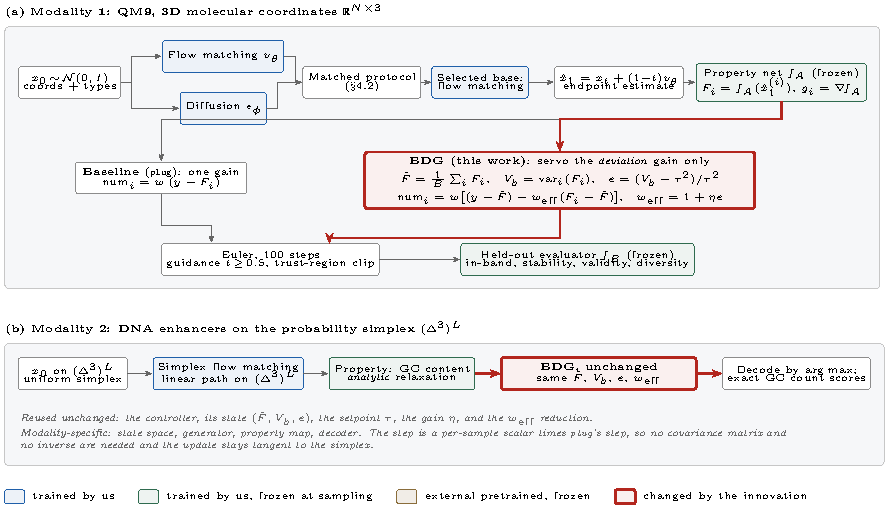
\includegraphics[width=0.60\linewidth]{figs/overview.pdf}
  \caption{Study overview. \textbf{(a)} Modality 1: one representation feeds a
  flow-matching and a diffusion model; the plug-in baseline applies one gain to
  $(y-F_i)$, BDG holds the centring gain at $w$ and servoes only $\weff$.
  \textbf{(b)} Modality 2: the controller transfers unchanged. Colour marks trained,
  frozen, pretrained, and changed-by-the-innovation components.}
  \label{fig:overview}
\end{figure}

\section{Results}

\subsection{Evaluation Protocol}
\label{sec:protocol}

The target metric is \ib, the fraction of molecules whose property, scored by the
held-out $f_B$, lies within $\pm\delta$ of the target, with $\delta=2\times$ the
evaluator's calibration mean absolute error on 3{,}000 disjoint molecules. We report
\ib{} decoded, the decomposition $\mathrm{RMSE}^2=\mathrm{bias}^2+\mathrm{spread}^2$ in
units of $\delta$, and the spread ratio against unguided, all at the \textbf{q50}
target. Arms share the checkpoint, guide, evaluator, target, atom counts and noise,
paired within a backend at $w=1$; equal $w$ is not equal force, the applied-correction
share spanning $5.8\times$. The headline uses three seeds.

\subsection{Modality 1: Flow Matching versus Diffusion}
\label{sec:fmvd}

\begin{table}[!tb]
\centering\tiny
\setlength{\tabcolsep}{4pt}
\caption{Base models on QM9, unconditional, 100-step Euler probability-flow ODE,
our evaluator under EDM conventions. Our flow row is three seeds of 10{,}000 samples;
\texttt{EDMsecond} is borrowed, $n{=}2{,}000$, one seed, so it is not comparable.
\pend{} marks a value the v3 run has not produced (Appendix~A.6).}
\label{tab:fmvd}
\begin{tabular}{llrrrrrr}
\toprule
Model & Source & Atom stab.$\uparrow$ & Mol.\ stab.$\uparrow$ & Validity$\uparrow$ & Uniq.$\uparrow$ & NFE$\downarrow$ & Params \\
\midrule
Flow matching (ours)          & reproduced & $0.9366$ & $0.3993$ & $0.7625$ & $0.9939$ &  $100$ & $3.75$\,M \\
VP diffusion (ours)           & reproduced & \pend    & \pend    & \pend    & \pend    &  $101$ & $3.75$\,M \\
\midrule
\texttt{EDMsecond} \citep{hoogeboom2022equivariant} & borrowed & $0.9644$ & $0.6725$ & $0.8490$ & \pend & $100$ & $5.34$\,M \\
EDM \citep{hoogeboom2022equivariant} & quoted & $0.9870$ & $0.8200$ & $0.9190$ & $-$ & $1000$ & $-$ \\
Real QM9 (ceiling)            & measured   & $0.9940$ & $0.9560$ & $0.9820$ & $1.0000$ & $-$ & $-$ \\
\bottomrule
\end{tabular}
\end{table}

In Table~\ref{tab:fmvd} our flow model reaches $0.9366$ atom and $0.3993$
molecule stability at 100 evaluations, saturating by 500 steps. Ranking the causes of the gap to published
equivariant diffusion: unscaled one-hot features lead, the published ablation losing 3
atom and 35 molecule points; then budget, 303k steps against roughly 1.56M; the
half-data split is ruled out at $0.33$ atom points, and the evaluator by bond tables
matching the reference. We carry flow matching forward without a fidelity win, since
the matched diffusion row is pending, and its linear path supplies the endpoint
estimate. \TODO{restate when v3 Job A lands}

\subsection{Modality 1: Guidance Works}
\label{sec:guidworks}

\begin{table}[!tb]
\centering\tiny
\setlength{\tabcolsep}{4.5pt}
\caption{Guided against unguided at q50, otherwise matched. One generator, one seed,
$n{=}256$, best strength per arm, no chemistry floor. Cells are $\mu$ / gap / $\alpha$.}
\label{tab:guidance}
\begin{tabular}{lrrr}
\toprule
Arm & \ib$\uparrow$ & Spread\,/\,unguided & Mol.\ stab.$\uparrow$ \\
\midrule
unguided                  & $0.090$\,/\,$0.121$\,/\,$0.051$ & $1.00$\,/\,$1.00$\,/\,$1.00$ & $0.434$\,/\,$0.434$\,/\,$0.434$ \\
plug-in (best $w$)        & $0.184$\,/\,$0.219$\,/\,$\mathbf{0.133}$ & $0.52$\,/\,$0.60$\,/\,$0.47$ & $0.246$\,/\,$0.199$\,/\,$0.320$ \\
TFG ($w{=}4$, $\mu$ only) & $\mathbf{0.535}$\,/\,$-$\,/\,$-$ & $0.22$\,/\,$-$\,/\,$-$ & $0.172$\,/\,$-$\,/\,$-$ \\
BDG ($w{=}32$)            & $0.180$\,/\,$\mathbf{0.227}$\,/\,$0.106$ & $0.49$\,/\,$0.68$\,/\,$0.53$ & $\mathbf{0.348}$\,/\,$0.262$\,/\,$0.340$ \\
\bottomrule
\end{tabular}
\end{table}

In Table~\ref{tab:guidance} guidance raises \ib{} by $2.0\times$ on $\mu$,
$1.9\times$ on the gap and $2.6\times$ on $\alpha$ for the plug-in rule, and TFG reaches $6.0\times$ on $\mu$. Molecule
stability falls from $0.434$ to $0.246$ for the plug-in rule and to $0.172$ for
TFG. Spread contracts to between $0.22$ and $0.60$: the arm that contracts most wins
\ib{} and loses the most chemistry.

\subsection{Modality 1: Innovation Ablations}
\label{sec:ablations}

\begin{table}[!tb]
\centering\tiny
\setlength{\tabcolsep}{4pt}
\caption{BDG ablations at q50, ordered by \emph{measured} $\weff$. Rows above the rule
are gates, below are controls. Port cells: $n{=}256$, one seed, $w{=}1$; the
three-seed v3 grid is in Appendix~A.3. \TODO{v3 ablation stage}}
\label{tab:ablation}
\begin{tabular}{llrrrrr}
\toprule
Variant & Role & $\eta$ & $\tau_{\mathrm{mult}}$ & Spread\,/\,ung. & \ib$\uparrow$ & Mol.\ stab.$\uparrow$ \\
\midrule
plug-in, $w{=}1$       & base    & $-$ & $-$   & $0.714$ & $0.1094$ & $0.3633$ \\
BDG $\eta{=}0$         & gate    & $0$ & $1.0$ & $0.714$ & $0.1094$ & $0.3633$ \\
BDG one-sided, expand  & gate    & $4$ & $1.5$ & $0.714$ & $0.1094$ & $0.3633$ \\
\midrule
BDG contract           & ladder  & $4$ & $0.5$ & $0.670$ & $0.1406$ & $0.3359$ \\
BDG neutral            & ladder  & $4$ & $1.0$ & $0.900$ & $0.0820$ & $0.4258$ \\
BDG expand             & ladder  & $4$ & $1.5$ & $1.093$ & $0.0703$ & $0.4141$ \\
\midrule
plug-in, $w{=}4$       & control & $-$ & $-$   & $0.584$ & $0.1406$ & $0.2656$ \\
open-loop $e$ replay   & control & $4$ & $0.5$ & $0.686$ & \pend    & \pend    \\
signed-$w$ plug-in     & control & $-$ & $-$   & \pend   & \pend    & \pend    \\
\bottomrule
\end{tabular}
\end{table}

\textbf{The gates pass exactly} in Table~\ref{tab:ablation}. At $\eta=0$ BDG is
bit-identical to the plug-in rule;
the one-sided variant likewise, its raw pre-clamp error of $-0.984$ clamped to $0$.
\textbf{The setpoint moves spread monotonically} on six of six curves, $0.670$ to
$1.219$ times unguided; the deviation gain changes sign up to 34 times and spans
$[-2.64,+10.35]$ against the bound $\weff\ge-3$. \textbf{Coverage does not improve.}
No rung beats the plug-in rule at $|z|\ge3$: over 72 paired tests the largest is
$3.07$, a \v{S}id\'ak-corrected $p=0.14$. \textbf{The controls.} Plug-in at $w=4$
matches BDG's contraction rung at $0.1406$ \ib{} on $0.2656$ molecule stability against
BDG's $0.3359$; the open-loop replay recovers 69.5\% to 96\% of the closed loop against
plug-in's 8.4\% to 30.5\% gap.

\subsection{Modality 1: Comparison with Recent Methods}
\label{sec:recent}

\begin{table}[!tb]
\centering\tiny
\setlength{\tabcolsep}{4pt}
\caption{Five recent inference-time guidance methods, all reproduced on our frozen
checkpoint, guide and evaluator at q50 and $w{=}1$. Passes are per cell, $n{=}5{,}000$.}
\label{tab:recent}
\begin{tabular}{llrrrrr}
\toprule
Method & Status & \ib$\uparrow$ & Mol.\ stab.$\uparrow$ & Diversity$\uparrow$ & Gen.\ passes & Guide passes \\
\midrule
DPS-style plug-in \citep{chung2023dps}  & reproduced & \pend & \pend & \pend & $10{,}000$ & $4{,}000$ \\
TMPD-inspired \citep{boys2024tmpd}      & reproduced & \pend & \pend & \pend & $10{,}000$ & $4{,}000$ \\
LGD-MC \citep{song2023lgd}              & reproduced & \pend & \pend & \pend & $12{,}000$ & $20{,}000$ \\
TFG \citep{ye2024tfg}                   & reproduced & \pend & \pend & \pend & $8{,}000$  & $20{,}000$ \\
D-Flow \citep{benhamu2024dflow}         & reproduced & \pend & \pend & \pend & \pend      & \pend \\
\midrule
Flow matching, unguided                 & internal   & \pend & \pend & \pend & $10{,}000$ & $0$ \\
\textbf{BDG (ours)}                     & reproduced & \pend & \pend & \pend & $10{,}000$ & $4{,}000$ \\
\bottomrule
\end{tabular}
\end{table}

Table~\ref{tab:recent} compares guidance rules on one frozen generator.
Appendix~A.4 records three port caveats. BDG uses $4{,}000$ guide passes
per cell against $20{,}000$ for LGD-MC and TFG. \TODO{better/comparable/worse discussion}

\subsection{Modality 2: Transfer of the Innovation}
\label{sec:m2}

\begin{table}[!tb]
\centering\tiny
\setlength{\tabcolsep}{5pt}
\caption{Transfer to DNA enhancers on the simplex. Signatures are exact statements about
the controller. Our base generator is the linear flow-matching model these papers
baseline against, so their numbers are never pooled with ours.}
\label{tab:m2}
\begin{tabular}{lcc}
\toprule
Signature & QM9 & DNA simplex \\
\midrule
$\eta{=}0$ reproduces plug-in & bit-identical & bit-identical \\
one-sided at an expanding setpoint & exact & exact, $\weff{=}{+}1.000$ \\
setpoint ladder monotone in spread & $0.67\!\to\!1.22$ & $0.81\!\to\!1.01$ \\
cost identical to plug-in & yes & yes, byte-identical \\
contraction breaks the fidelity floor & yes & yes \\
\ib{} improves & no & no \\
\midrule
\multicolumn{3}{l}{\emph{Against recent simplex sequence models}}\\
Dirichlet FM \citep{stark2024dirichlet} & \multicolumn{2}{c}{\TODO{v3 Job B}} \\
Fisher Flow \citep{davis2024fisher} & \multicolumn{2}{c}{\TODO{v3 Job B}} \\
MOG-DFM \citep{chen2025mogdfm} & \multicolumn{2}{c}{\TODO{v3 Job B}} \\
\textbf{BDG, transferred (ours)} & \multicolumn{2}{c}{\TODO{v3 Job B}} \\
\bottomrule
\end{tabular}
\end{table}

In Table~\ref{tab:m2} BDG transferred with no change to the controller, and
coverage does not improve. The
effect is $2.6\times$ smaller, $0.20$ against $0.52$: GC is affine in the simplex
coordinates, it averages over 200 positions, and the band spans only $4.3$ attainable
values at granularity $1/200$.

\subsection{Cross-Modality Analysis and Failure Modes}
\label{sec:failure}

The direction matches across modalities and the magnitude does not, which the property
map explains. Two measured confounds bound the result. The trade-off is
re-parameterised and not removed: chemistry cost tracks $|\weff|$, a correlation over
coupled cells. The trust region is a live confound at large $|\weff|$, the plug-in rule
clipping on 884 sample steps where the contracting rung clips on 2{,}516, so a rung can
be clip-limited and not controller-limited.

\section{Discussion}

Flow matching carries the study for its endpoint estimate and not a fidelity win,
guidance works at a measured chemistry cost, and the ablations give one causal
statement, that the dispersion term and only it produces the spread ladder, beside one
null on coverage. Both transfer to the simplex.

Equation~\eqref{eq:reduction} explains the null: BDG is the plug-in field at a rescaled
weight aiming at a shifted target, so it cannot exceed what that field reaches. The
centring gain stays at $w$ while the deviation gain is set online and may pass through
zero, which is the one place BDG is ahead: more chemistry at matched coverage.

Three limitations bound the claim, each naming its next experiment: the trust region
confounds the largest rungs, the signed-$w$ control has not run, and the open-loop
control rests on one seed pair. The narrowest claim supported is monotone, two-sided,
modality-portable spread control at no extra sampling cost, which converts the
coverage-against-fidelity trade-off into a quantity the user requests.
